\documentclass[11pt]{article}

\usepackage{fontspec}
\usepackage[brazilian]{babel}
\usepackage[a4paper,margin=2.5cm]{geometry}
\usepackage{amsmath}
\usepackage{graphicx}
\usepackage{booktabs}
\usepackage{listings}
\usepackage{xurl}
\usepackage{hyperref}
\hypersetup{colorlinks=false, pdfborder={0 0 0}}

\setlength{\parskip}{0.4em}
\setlength{\parindent}{0pt}

\lstset{
  basicstyle=\ttfamily\footnotesize,
  frame=single,
  framerule=0.3pt,
  breaklines=true,
  columns=fullflexible,
  keepspaces=true,
  showstringspaces=false,
  numbers=left,
  numberstyle=\tiny,
  xleftmargin=2em,
  belowskip=0.6em,
  aboveskip=0.6em,
}

\title{\vspace{-1.5cm}\bfseries ephemnous: escalonamento por aprendizado de m\'aquina para data centers em \'orbita baixa}
\date{}

\begin{document}

\begin{center}
{\LARGE\bfseries ephemnous}\\[0.3em]
{\large Escalonamento por aprendizado de m\'aquina para data centers em \'orbita baixa}\\[1.2em]
{\large Karina Queiroz de Gennaro (RM570928)}\\
{\large Luis Felipe Bardi (RM569479)}\\
{\large Beatriz de Oliveira Ossola Ribeiro (RM570190)}\\[0.8em]
{\large FIAP Global Solution}\\[1.2em]
{\Large\bfseries QUERO CONCORRER}\\[1.0em]
\today
\end{center}

\vspace{0.5em}

\begin{abstract}
\noindent
Data centers em \'orbita baixa deixaram de ser fic\c{c}\~ao: em 2025, projetos como Starcloud e o Google Project Suncatcher colocaram (ou anunciaram) computa\c{c}\~ao em \'orbita. L\'a, a energia solar oscila (o sat\'elite entra na sombra da Terra a cada $\sim$95 min) e o calor s\'o sai por radia\c{c}\~ao, porque no v\'acuo n\~ao h\'a convec\c{c}\~ao. Apresentamos o \textbf{ephemnous}, um escalonador que prev\^e a energia e a folga t\'ermica das pr\'oximas janelas e decide o que computar: rodar no sol, fazer \emph{checkpoint} antes do eclipse e dar \emph{throttle} para n\~ao superaquecer. Um \emph{forecaster} de \emph{gradient boosting} prev\^e energia e folga t\'ermica; um controlador preditivo (MPC) decide a partir das previs\~oes. Medimos com honestidade: a previs\~ao supera um baseline reativo justo de forma \textbf{robusta apenas no regime energia-cr\'itico} (ganho de 20--25\% em \emph{jobs} conclu\'idos, intervalo de confian\c{c}a de 95\% acima de zero em tr\^es blocos de sementes) e \textbf{empata quando h\'a folga de bateria}. O sistema roda ponta a ponta: ESP32 simulado no Wokwi, backend FastAPI, banco PostgreSQL e \emph{dashboard}.
\end{abstract}

\section{Introdu\c{c}\~ao}

A demanda por computa\c{c}\~ao cresce mais r\'apido que a capacidade de aliment\'a-la e refriger\'a-la na Terra. Uma resposta emergente \'e levar data centers para a \'orbita, onde h\'a energia solar abundante e um sumidouro t\'ermico frio. O conceito saiu do papel em 2025 com iniciativas como Starcloud e Google Project Suncatcher, mas n\~ao existe um demonstrador acess\'ivel do \emph{escalonamento} dessa carga.

O ambiente orbital imp\~oe dois problemas sem an\'alogo no solo:

\begin{itemize}
\item \textbf{Energia intermitente.} Em \'orbita baixa o per\'iodo \'e de cerca de 95 minutos e parte dele \'e passada na sombra da Terra (eclipse), quando o painel n\~ao gera nada.
\item \textbf{Calor s\'o por radia\c{c}\~ao.} No v\'acuo n\~ao h\'a convec\c{c}\~ao; o calor gerado pela computa\c{c}\~ao s\'o sai irradiando, de forma lenta e n\~ao linear (lei de Stefan-Boltzmann).
\end{itemize}

Decidir o que computar a cada instante, sob essas restri\c{c}\~oes, \'e um problema de escalonamento ciente de energia e temperatura. O ephemnous ataca esse problema e, mais importante, \emph{mede honestamente} quando a previs\~ao agrega valor. O projeto se alinha aos ODS 9 (ind\'ustria, inova\c{c}\~ao e infraestrutura) e 13 (a\c{c}\~ao clim\'atica).

A contribui\c{c}\~ao n\~ao \'e ``nossa IA vence sempre''. \'E um sistema completo, reprodut\'ivel e barato, com uma avalia\c{c}\~ao rigorosa que mostra \emph{onde} prever ganha de reagir, e onde n\~ao ganha.

\section{Desenvolvimento}

\subsection{Vis\~ao geral da solu\c{c}\~ao}

O ephemnous \'e um la\c{c}o fechado: um n\'o de borda reporta telemetria; o \emph{backend} avan\c{c}a a f\'isica, prev\^e o futuro pr\'oximo, decide a a\c{c}\~ao e devolve o comando. A f\'isica orbital, t\'ermica e de bateria vive em um \'unico m\'odulo Python, compartilhado pela demonstra\c{c}\~ao ao vivo, pela frota simulada e pela gera\c{c}\~ao de dados de treino. Isso elimina diverg\^encia entre demo e treino.

\subsection{Arquitetura}

A Figura~\ref{fig:arq} mostra os componentes. O n\'o de borda \'e um ESP32 simulado no Wokwi: l\^e um potenci\^ometro (irradi\^ancia solar e gatilho de eclipse) e um bot\~ao, atua um LED por PWM (a carga de computa\c{c}\~ao vis\'ivel) e troca dados por HTTP. O backend FastAPI \'e o dono da escrita no PostgreSQL e roda o \emph{forecaster} e o MPC. Uma frota simulada de N n\'os e a gera\c{c}\~ao de dados usam a mesma f\'isica.

\begin{figure}[h]
\centering
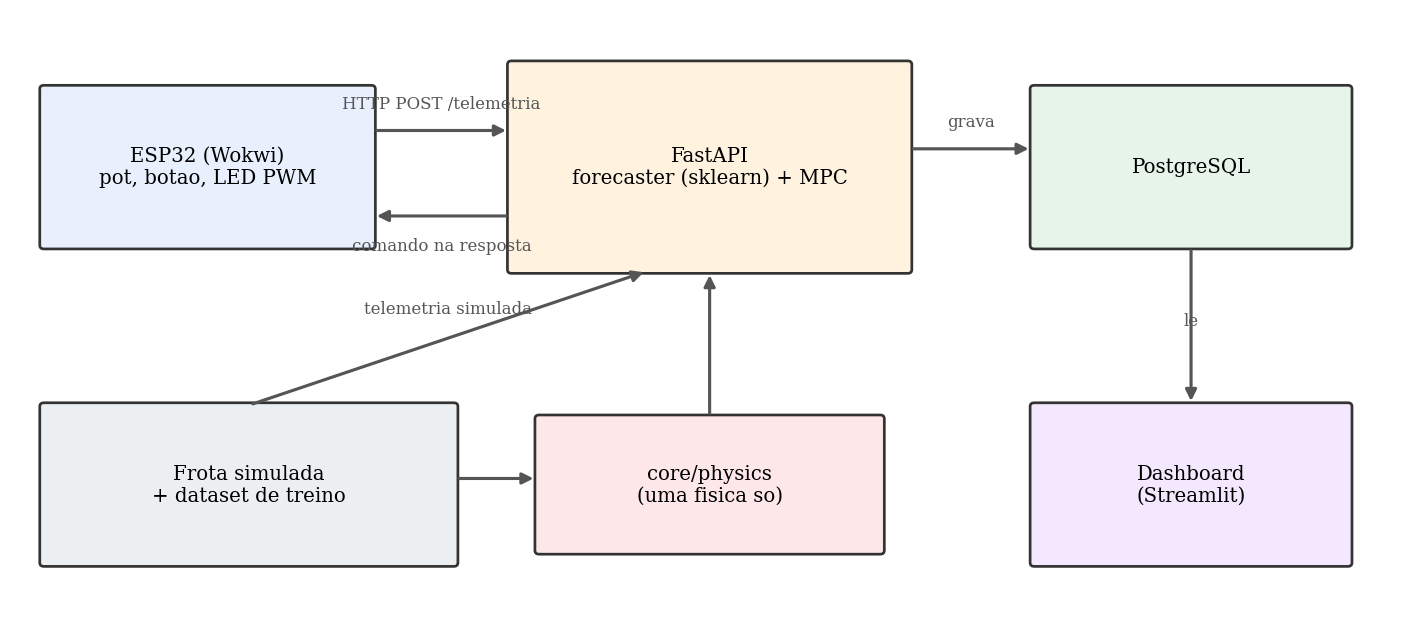
\includegraphics[width=0.95\textwidth]{fig_arquitetura.png}
\caption{Arquitetura do ephemnous. A f\'isica fica s\'o no backend; o ESP32 \'e um n\'o fino que sente e atua.}
\label{fig:arq}
\end{figure}

\textbf{Decis\~ao: onde a f\'isica mora.} Optamos por mant\^e-la \emph{s\'o no backend} (n\~ao no firmware), o que evita duplicar e dessincronizar a f\'isica entre C++ e Python. \'E tamb\'em fisicamente honesto: um sat\'elite real n\~ao ``calcula'' a irradi\^ancia que recebe; isso \'e o mundo. O ESP32 contribui com leitura de sensor e atua\c{c}\~ao.

\subsection{Simulador e f\'isica}

O rel\'ogio orbital usa a terceira lei de Kepler, $T = 2\pi\sqrt{a^3/\mu}$, com $a = R_{\oplus} + h$. A fra\c{c}\~ao de \'orbita em eclipse, para um \^angulo $\beta$, \'e
\[
f_{ecl} = \frac{1}{\pi}\arccos\!\left(\frac{\sqrt{h^2 + 2 R_{\oplus} h}}{(R_{\oplus}+h)\cos\beta}\right).
\]
A temperatura segue um balan\c{c}o t\'ermico de massa concentrada, integrado por Euler:
\[
C\,\frac{dT}{dt} = Q_{comp} + Q_{solar} - \varepsilon\,\sigma\,A\,(T^4 - T_{sink}^4),
\]
onde $\sigma$ \'e a constante de Stefan-Boltzmann. A bateria integra a pot\^encia l\'iquida, $dE/dt = P_{gen} - P_{draw}$, e o estado de carga \'e $\mathrm{SoC} = E/E_{cap}$. O n\'ucleo desse passo \'e direto:

\begin{lstlisting}[language=Python]
q_solar = p.absorptivity * p.s_solar_w_m2 * p.a_panel_m2 * eff
q_comp  = load * p.q_comp_max_w
q_rad   = p.emissivity * SIGMA * p.a_rad_m2 * (state.temp_k**4 - p.t_sink_k**4)
temp    = state.temp_k + (p.dt_s / p.c_thermal_j_k) * (q_comp + q_solar - q_rad)

p_gen   = p.panel_eff * p.s_solar_w_m2 * p.a_panel_m2 * eff
p_draw  = p.p_base_w + load * p.p_comp_max_w
energy_j = clamp(state.soc_frac * e_cap_j + (p_gen - p_draw) * p.dt_s, 0.0, e_cap_j)
soc      = energy_j / e_cap_j
\end{lstlisting}

\subsection{Coleta de dados e banco}

O ESP32 envia telemetria por \texttt{POST /telemetry} e recebe o comando na resposta do mesmo POST (um \emph{round-trip} fecha o la\c{c}o; escolhemos HTTP em vez de MQTT porque um n\'o real mais a frota simulada n\~ao justifica um \emph{broker}). O PostgreSQL guarda n\'os, telemetria, estado f\'isico, previs\~oes, decis\~oes e \emph{jobs}. As unidades s\~ao can\^onicas: pot\^encia em Watts, temperatura em Kelvin, fra\c{c}\~oes em $[0,1]$, com a convers\~ao para Kelvin feita no firmware antes do envio.

\subsection{Modelos de IA}

\textbf{Forecaster (o aprendizado).} Um \texttt{HistGradientBoostingRegressor} (scikit-learn) prev\^e, para horizontes de 1 a 5 passos, a pot\^encia dispon\'ivel e a folga t\'ermica. As \emph{features} usam apenas informa\c{c}\~ao em $t$ ou antes (defasagens de pot\^encia, temperatura e carga; estat\'isticas m\'oveis; \emph{features} c\'iclicas de fase). Contra vazamento (\emph{leakage}): os r\'otulos v\^em de um \emph{rollout} limpo, as \emph{features} v\^em de observa\c{c}\~oes com ru\'ido de sensor, e a divis\~ao treino/valida\c{c}\~ao \'e por epis\'odio. Um fator estoc\'astico de apontamento/atitude (passeio aleat\'orio) torna o futuro n\~ao determin\'avel apenas pela efem\'eride.

\textbf{Escalonador (MPC heur\'istico).} O controlador consome as previs\~oes e decide entre rodar, adiar, fazer \emph{checkpoint} ou \emph{throttle}. O baseline ``reativo'' \'e o \emph{mesmo c\'odigo} com horizonte zero, o que torna a compara\c{c}\~ao justa por constru\c{c}\~ao.

\begin{lstlisting}[language=Python]
if fut_margin < MARGIN_CRIT_K:
    return Decision("throttle", 40, ...)        # folga termica critica prevista
if eclipse_soon and state.soc_frac < CHECKPOINT_SOC:
    return Decision("checkpoint", 0, ...)       # salva antes de perder energia
if state.power_avail_w < p.p_base_w and state.soc_frac < SOC_LOW:
    return Decision("defer", 0, ...)            # sem energia, adia
if fut_margin < MARGIN_LOW_K:
    return Decision("throttle", 128, ...)       # folga moderada, meia carga
return Decision("run", 255, ...)                # tudo folgado, plena carga
\end{lstlisting}

\subsection{Decis\~oes do grupo}

\begin{itemize}
\item \textbf{Arquitetura limpa, sem DDD.} Camadas \texttt{core} (puro), \texttt{services} (orquestra\c{c}\~ao) e \texttt{infra} (FastAPI, Postgres, ML), com a regra de depend\^encia apontando para dentro.
\item \textbf{Wokwi em vez de placa f\'isica.} Remove solda e calibra\c{c}\~ao, e o gatilho ao vivo (potenci\^ometro/bot\~ao) \'e mais confi\'avel que uma l\^ampada real.
\item \textbf{Heur\'istica em vez de RL/Deep Learning.} A pol\'itica \'otima \'e simples e o \emph{gradient boosting} j\'a est\'a no teto pr\'atico de previsibilidade; avaliamos RL e \emph{deep learning} e os descartamos com justificativa (ver Conclus\~oes).
\item \textbf{Admiss\~ao ciente de risco.} Para \emph{jobs} n\~ao interromp\'iveis, a decis\~ao de iniciar simula o estado de carga ao longo da dura\c{c}\~ao do \emph{job}; essa corre\c{c}\~ao estrutural foi o que tornou a vantagem da previs\~ao robusta.
\end{itemize}

\subsection{Dashboard e demonstra\c{c}\~ao}

O \emph{dashboard} (Streamlit) mostra telemetria ao vivo, a curva de previs\~ao, as decis\~oes da IA e o comparativo. A Figura~\ref{fig:tel} ilustra uma \'orbita: a pot\^encia cai no eclipse, a previs\~ao (tracejada) antecipa a queda, a temperatura fica sob o limite e a bateria drena e recarrega; o MPC faz \emph{checkpoint} antes de a energia acabar. O gatilho ao vivo: baixar o potenci\^ometro provoca o eclipse, o LED escurece e a decis\~ao aparece no banco com \texttt{model\_version=hgb}.

\begin{figure}[h]
\centering
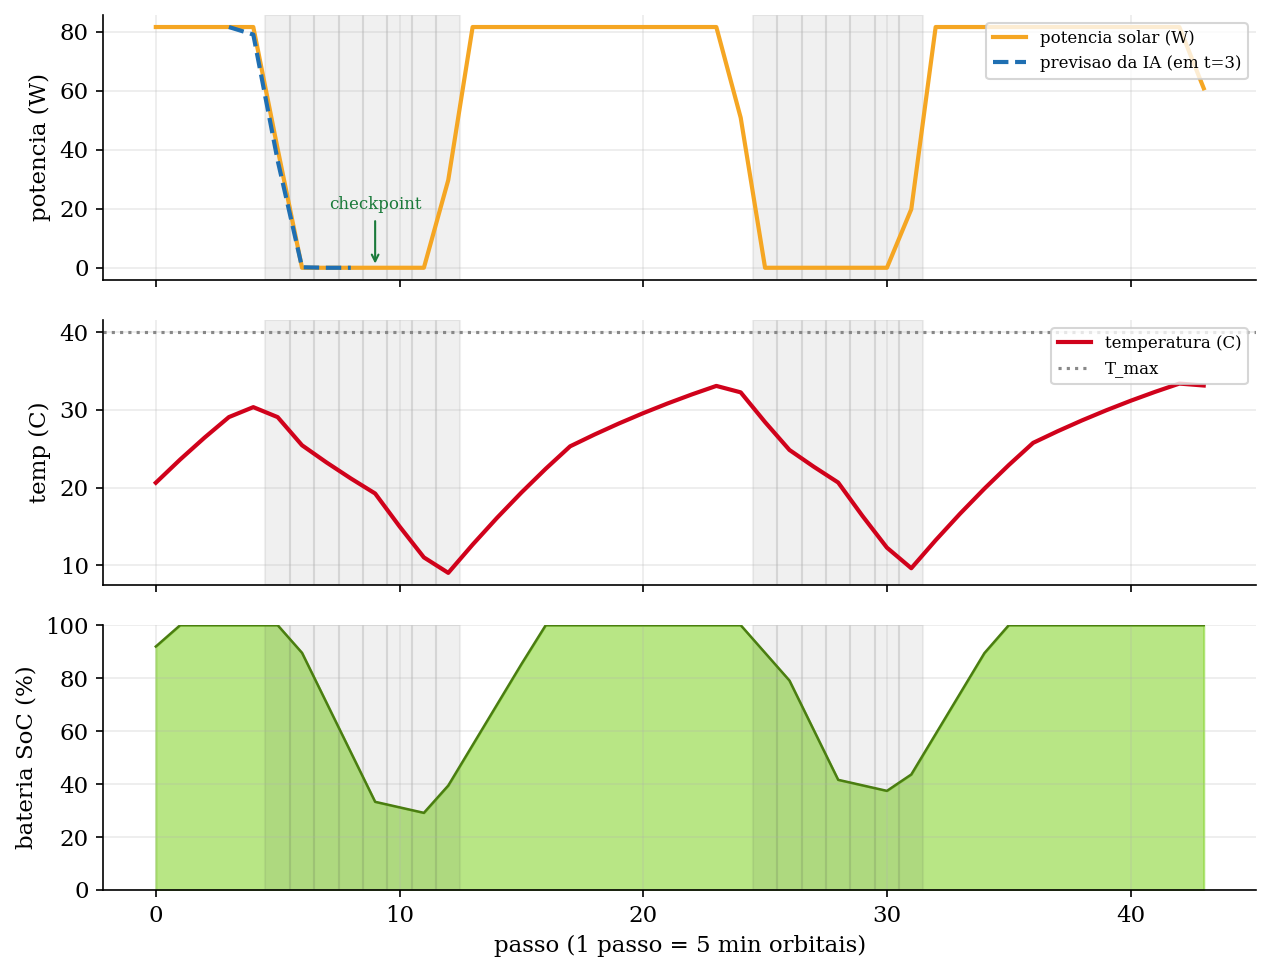
\includegraphics[width=0.92\textwidth]{fig_telemetria.png}
\caption{Telemetria e decis\~ao da IA ao longo de duas \'orbitas (faixas em cinza s\~ao eclipses).}
\label{fig:tel}
\end{figure}

A Figura~\ref{fig:dash} mostra o \emph{dashboard} em execu\c{c}\~ao durante um eclipse: a pot\^encia caiu, a previs\~ao (tracejada, em azul) aponta para baixo e a \'ultima decis\~ao da IA \'e \emph{checkpoint}.

\begin{figure}[h]
\centering
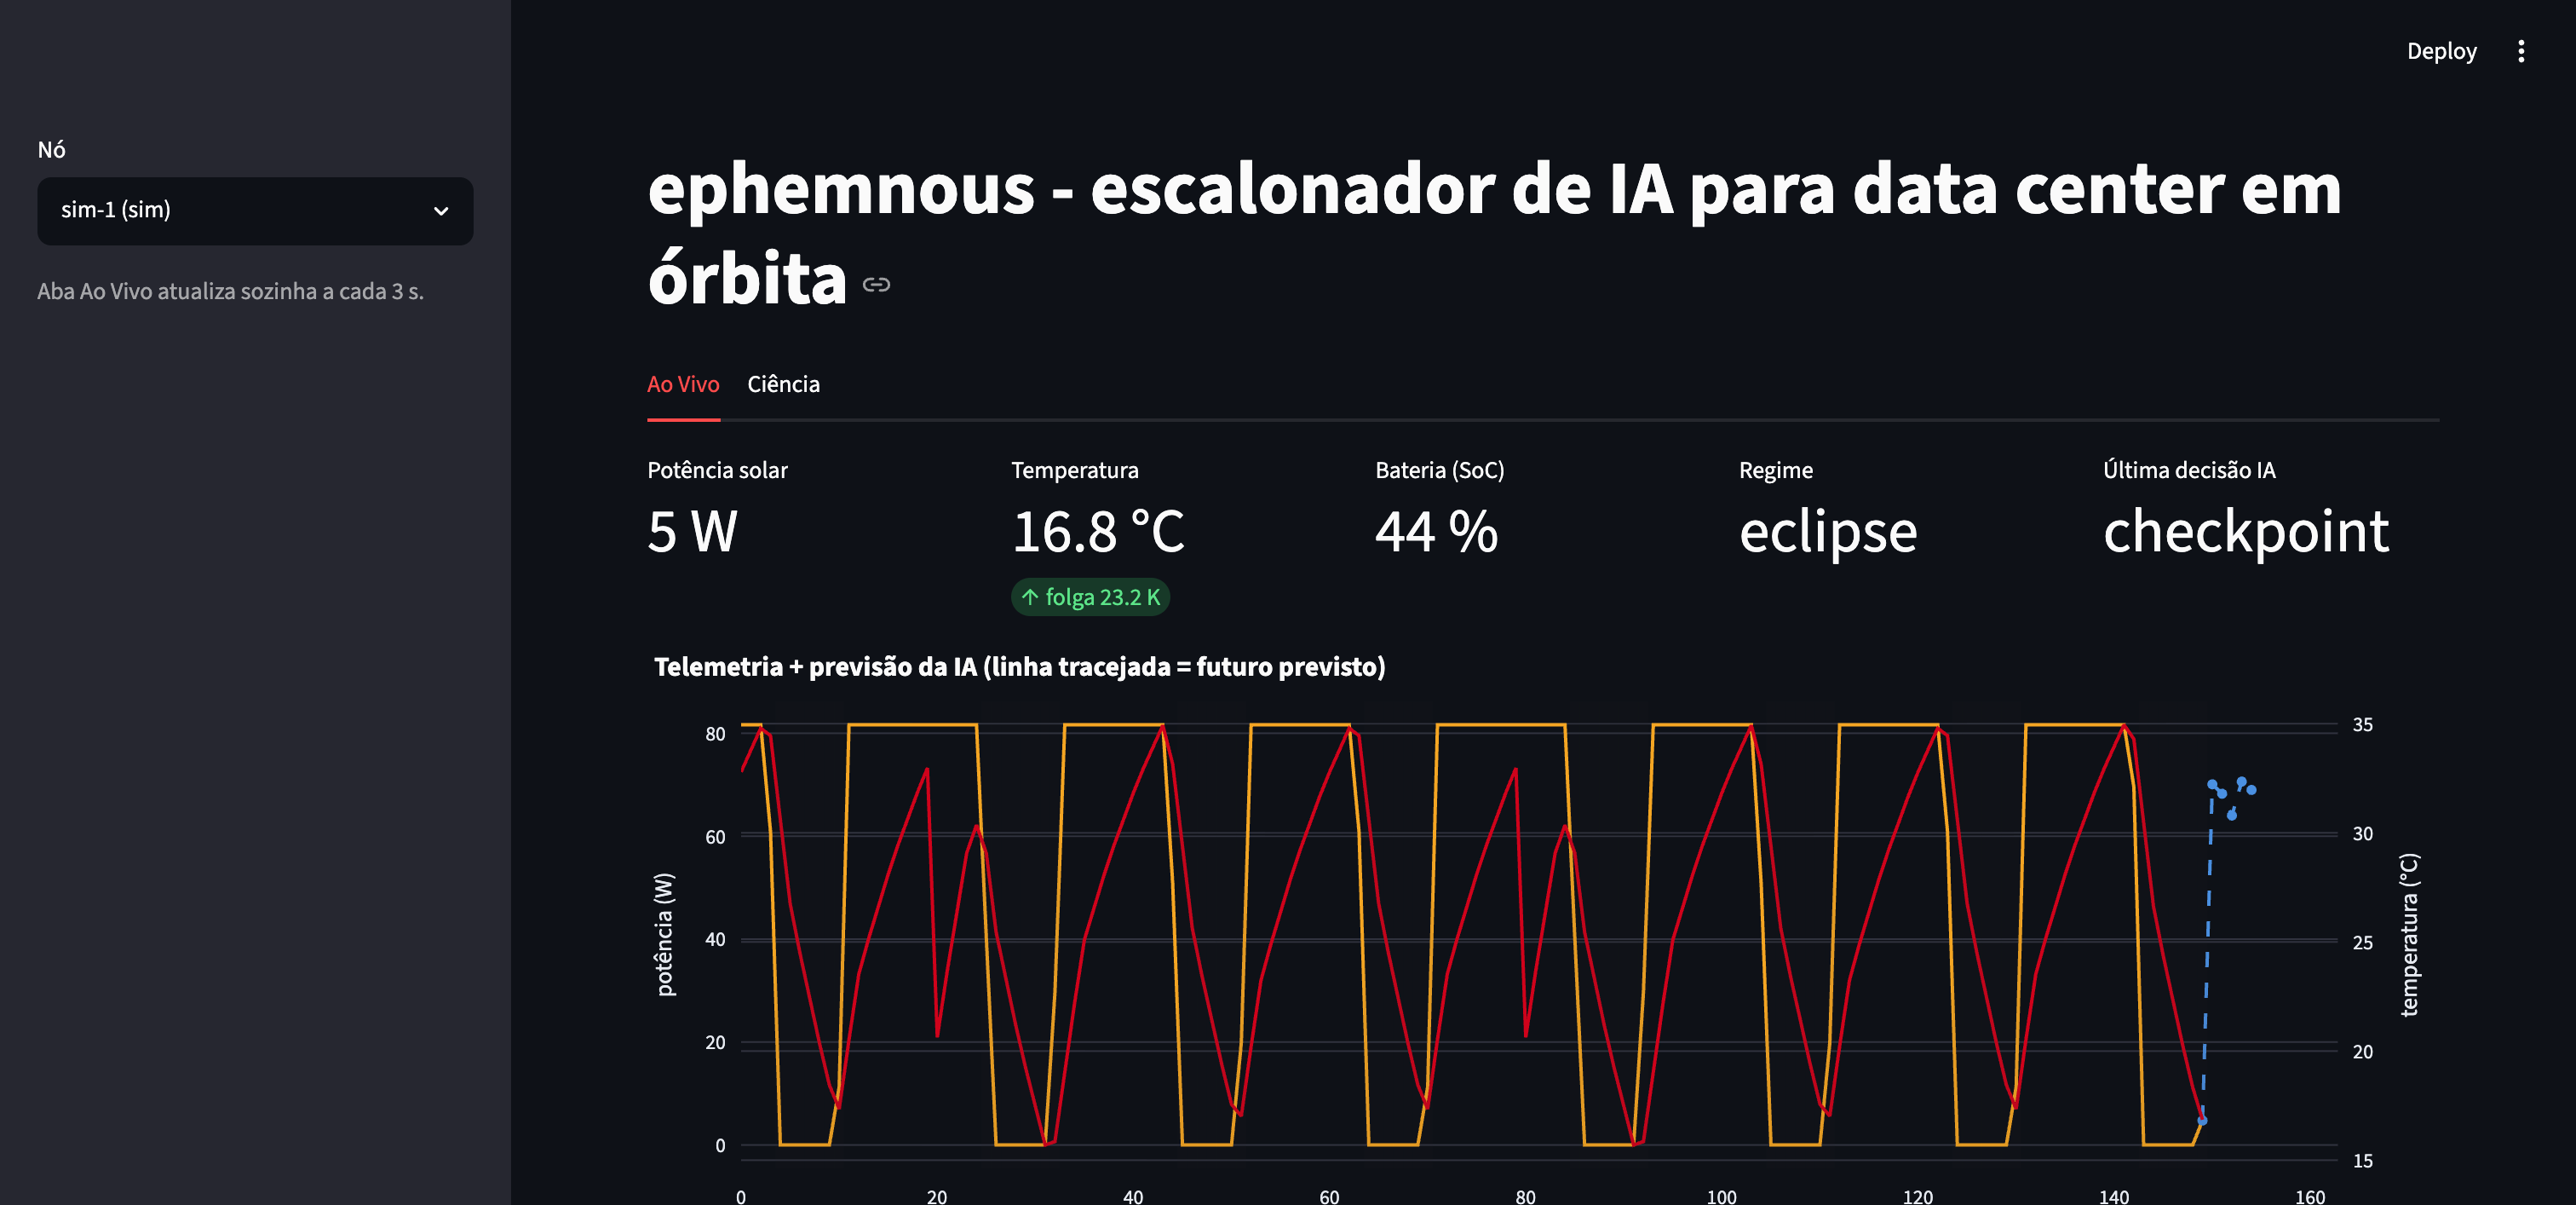
\includegraphics[width=0.95\textwidth]{fig_dashboard.png}
\caption{Dashboard ao vivo (aba ``Ao Vivo''), com o n\'o em eclipse: m\'etricas, telemetria com a curva de previs\~ao e a \'ultima decis\~ao (\emph{checkpoint}).}
\label{fig:dash}
\end{figure}

\section{Resultados Esperados}

\subsection{O forecaster \'e aprendizado de verdade}

A Tabela~\ref{tab:skill} mostra o \emph{skill} (1 menos a raz\~ao de RMSE) contra dois baselines: persist\^encia inteligente (mesma fase, \'orbita anterior) e a \emph{efem\'eride pura} (pot\^encia nominal da \'orbita conhecida). O \emph{skill} positivo contra a efem\'eride prova que o modelo prev\^e a parte \emph{incerta} (apontamento), n\~ao o eclipse determin\'istico. O \emph{skill} cai com o horizonte, como esperado, e n\~ao \'e $\sim$1,0; se fosse, indicaria vazamento.

\begin{table}[h]
\centering
\begin{tabular}{lccccc}
\toprule
Alvo / horizonte (passos) & 1 & 2 & 3 & 4 & 5 \\
\midrule
Energia: skill vs persist\^encia & 0,68 & 0,67 & 0,66 & 0,65 & 0,64 \\
Energia: skill vs efem\'eride    & 0,78 & 0,71 & 0,67 & 0,63 & 0,60 \\
Folga t\'ermica: skill vs persist\^encia & 0,89 & 0,81 & 0,73 & 0,67 & 0,61 \\
\bottomrule
\end{tabular}
\caption{Skill do forecaster na valida\c{c}\~ao por epis\'odio. Sem vazamento (skill longe de 1,0; cai com o horizonte).}
\label{tab:skill}
\end{table}

\subsection{Quando prever ganha de reagir}

Para \emph{jobs} n\~ao interromp\'iveis (uma vez iniciado, ou termina ou \'e perdido se a bateria zerar), comparamos a admiss\~ao guiada pela previs\~ao do ML contra a guiada por persist\^encia, usando a \emph{mesma} regra de admiss\~ao. A m\'etrica \'e a pontua\c{c}\~ao l\'iquida (conclu\'idos menos duas vezes os perdidos). A Figura~\ref{fig:reg} \'e a curva de regime: a vantagem da IA \'e grande e robusta quando a bateria \'e apertada e desaparece quando h\'a folga.

\begin{figure}[h]
\centering
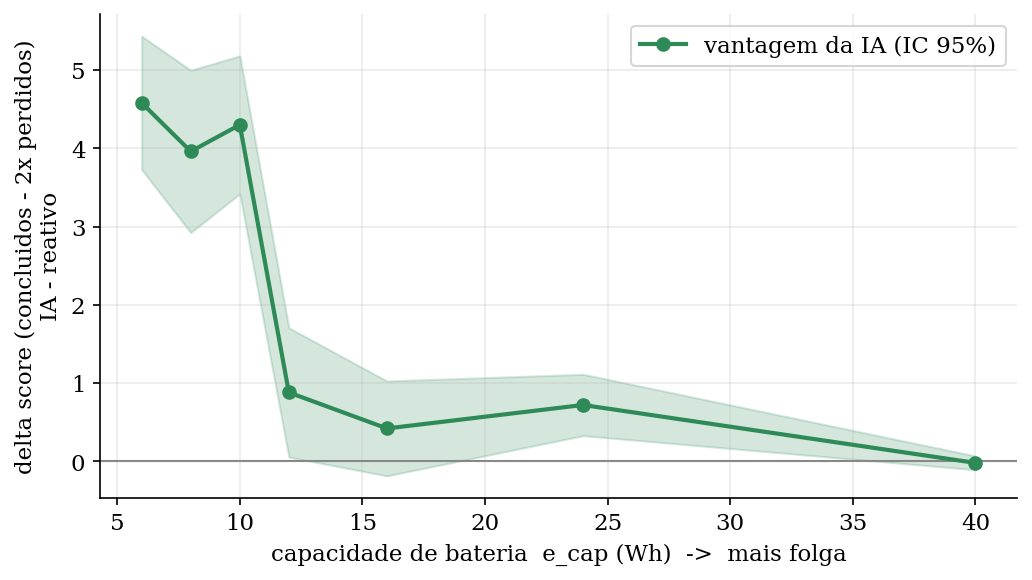
\includegraphics[width=0.78\textwidth]{fig_regime.png}
\caption{Vantagem da IA sobre o reativo (diferen\c{c}a de pontua\c{c}\~ao, com IC 95\% pareado) em fun\c{c}\~ao da capacidade de bateria. A vantagem concentra-se no regime energia-cr\'itico.}
\label{fig:reg}
\end{figure}

No regime energia-cr\'itico (bateria de 6 a 12 Wh), a IA conclui cerca de 20 a 25\% mais \emph{jobs} e perde de 65 a 75\% menos, com diferen\c{c}a de pontua\c{c}\~ao de $+3{,}3$ a $+4{,}9$ e intervalo de confian\c{c}a de 95\% acima de zero em tr\^es blocos de sementes independentes. Com bateria folgada ($\geq 16$ Wh), o resultado \'e um empate, e n\'os o reportamos. Uma abla\c{c}\~ao mostrou ainda que uma admiss\~ao excessivamente conservadora (quantil P10) zera o \emph{throughput}: aprendemos que o que importava era a corre\c{c}\~ao estrutural (simular o estado de carga ao longo do \emph{job}), n\~ao o quantil.

\subsection{Impacto esperado}

A leitura central \'e que \emph{a previs\~ao vale proporcionalmente ao custo do erro irrevers\'ivel}. Em um sat\'elite real, com restri\c{c}\~oes energ\'eticas apertadas e \emph{jobs} caros de refazer, esse regime \'e exatamente o esperado, o que sugere que o escalonamento preditivo \'e mais valioso na pr\'atica do que em uma simula\c{c}\~ao folgada. O sistema \'e barato, reprodut\'ivel e mensur\'avel, o que o torna uma base honesta para evoluir.

\section{Conclus\~oes}

Constru\'imos e demonstramos, de ponta a ponta, um conceito que hoje s\'o aparece em \emph{papers}: um escalonador de computa\c{c}\~ao orbital ciente de energia e temperatura, com ESP32, sensores, banco de dados e aprendizado de m\'aquina com papel central. Mais do que isso, medimos com rigor cient\'ifico \emph{onde} a previs\~ao agrega valor (regime energia-cr\'itico) e fomos transparentes sobre o empate no regime folgado.

\textbf{Por que n\~ao RL nem Deep Learning.} Avaliamos os dois. A pol\'itica \'otima do escalonador \'e uma \'arvore de poucas regras sobre duas vari\'aveis: um agente de \emph{reinforcement learning} no m\'aximo empata, ao custo de instabilidade e do risco de ajustar a recompensa (uma porta para resultados viciados). Para o \emph{forecaster}, com dataset pequeno e horizonte curto, o \emph{gradient boosting} j\'a est\'a no teto de previsibilidade imposto pela incerteza irredut\'ivel; \emph{deep learning} apenas sobreajustaria. Saber o que n\~ao usar \'e parte da engenharia.

\textbf{Limita\c{c}\~oes e trabalho futuro.} Os dados s\~ao simulados (de forma realista: \'orbita por Kepler, radia\c{c}\~ao de Stefan-Boltzmann, ru\'ido de sensor). O escalonamento usa uma carga sint\'etica; o pr\'oximo passo natural \'e uma fila combinat\'oria de N \emph{jobs} heterog\^eneos com prazos, regime em que uma pol\'itica aprendida (RL) ou de otimiza\c{c}\~ao pode finalmente superar a heur\'istica manual. Validar o \emph{forecaster} em hardware real (ESP32 f\'isico) tamb\'em est\'a no horizonte.

\section*{V\'ideo de demonstra\c{c}\~ao}

\noindent
Link do v\'ideo: \href{https://www.youtube.com/watch?v=GAs3oIsI3PU}{\url{https://www.youtube.com/watch?v=GAs3oIsI3PU}}

\noindent
Reposit\'orio do projeto:\\
\href{https://github.com/lfbardi-don/TEMPLATE-TIAO-2026/tree/main/1TIAO/Global-Solution-1}{\url{https://github.com/lfbardi-don/TEMPLATE-TIAO-2026/tree/main/1TIAO/Global-Solution-1}}

\begin{thebibliography}{9}
\bibitem{starcloud} Starcloud (anteriormente Lumen Orbit). Data centers em \'orbita, 2025.
\bibitem{suncatcher} Google. Project Suncatcher: explorando \emph{machine learning} no espa\c{c}o, 2025.
\bibitem{sklearn} Pedregosa et al. Scikit-learn: Machine Learning in Python. JMLR, 2011.
\end{thebibliography}

\end{document}
